\section{Three Stylized Facts}
\label{sec:stylized}

Before any estimation, three descriptive regularities frame the question.
Together they make the leverage-cycle reading a priori doubtful, which
is why the apparently confirming result of Section~\ref{sec:apparent}
deserves the scrutiny it receives in Section~\ref{sec:deconstruction}.

\paragraph{Fact 1.}
ETH's distribution is downside-asymmetric and fat-tailed, but the asymmetry is market-wide.
Hourly log returns have skewness \SkewEth{} and excess kurtosis \KurtEth{}
(Table~\ref{tab:descriptives}); the worst hour ($\MinRet\%$) is 1.7 times
deeper than the best ($+\MaxRet\%$); and far-extreme counts are
left-heavy, with \FarFiveDown{} hours at or below $-5\%$ against \FarFiveUp{}
at or above $+5\%$ (\FarSevenDown{} versus \FarSevenUp{} at $\pm 7\%$). The
measurement deserves precision, because the 1\% and 5\% \emph{quantiles}
themselves are nearly symmetric ($|p_1|/p_{99} = \QratioOnePct$): the
left-heaviness is a property of the far extremes, not of the moderate
tails. Heavy tails as such are the expected stylized fact
\citep{cont2001,osterrieder2017}, and the \emph{sign} of crypto skewness
varies with the return definition and sample: \citet{liu2021} report
positive skewness in simple returns across major cryptocurrencies, whereas
the hourly log returns studied here skew negative. Two further observations
discipline the interpretation. Negative jumps, a driver of volatility
documented across the major crypto markets \citep{ftiti2021}, are not
specific to ETH, and tail dependence
\emph{across} cryptocurrencies is, if anything, stronger on the upside
\citep{nguyen2020}. So nothing in Fact 1 licenses an attribution of the
asymmetry to DeFi. Figure~\ref{fig:distribution} displays the distribution.

\begin{figure}[t]
\centering
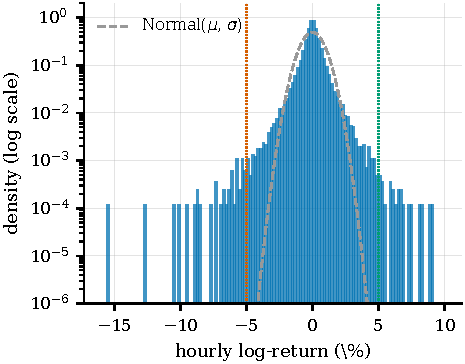
\includegraphics[width=0.55\textwidth]{../paper/figures/fig2_return_distribution}
\caption{Hourly ETH log returns (density, log scale) against a normal
benchmark. Dotted lines mark the $\pm 5\%$ far-extreme thresholds of
Table~\ref{tab:descriptives}.}
\label{fig:distribution}
\end{figure}

\paragraph{Fact 2.}
Liquidations are a mechanical marker of crashes, not evidence of causing them.
Among the worst 1\% of return hours, \PLiqWorstOne\% contain
contemporaneous liquidations, against \PLiqBestOne\% of the best 1\% and
\PLiqAll\% of all hours (Table~\ref{tab:descriptives}, Panel B).
The direction of this co-occurrence is mechanically determined. A price
fall pushes positions below their collateral threshold and triggers
liquidation, which is the protocol design \citep{qin2021,perez2021},
whereas a rally liquidates nothing. This asymmetry therefore
reflects the one-sidedness of the liquidation trigger, not downside
amplification of prices by DeFi. Consistently, \citet{moallemi2024}
document that over 70\% of liquidations occur in the absence of any
downward price jump, and pool-level price impacts of liquidations are small and temporary \citep{tian2025}. Fact 2 is the foundation of the paper's
register: at the hourly grain the liquidation--return relation is
bidirectional at short horizons, so every estimate below is read as
predictive association, never as a causal effect.

\paragraph{Fact 3.}
The observable flow is minute relative to the ETH market.
Median daily DeFi liquidations amount to roughly \SizeMedianShare{} of one percent
of estimated ETH spot-plus-perpetual turnover; the mean is
\SizeShareMean\%; and even the worst liquidation day of the sample reaches
only \SizeShareWorstDay\% (Table~\ref{tab:sizeratio} below reports the full
set). Against the largest reported centralized-exchange liquidation cascade on
record, roughly nineteen billion dollars in a single day
\citep{coinglass2025}, the typical daily flow sits four to six orders of
magnitude lower. The denominators are industry estimates, partly inflated
by wash trading and not peer-reviewed, so these are order-of-magnitude
bounds. But the inequality is wide enough to survive any plausible
rescaling, and the numerator is our own hard extraction. Fact 3 pre-loads the mechanism discussion of
Section~\ref{sec:mechanisms}: whatever the within-pool impact of an
individual liquidation, the aggregate observable flow is small relative to
the market that would need to be moved.

\medskip
\noindent
These three regularities, a real but market-wide asymmetry, mechanically
reverse co-occurrence, and negligible scale, make it doubtful from the
outset that observable DeFi liquidations drive ETH's downside tail. The
remainder of the paper tests that doubt formally: the next section fixes
the specification, Section~\ref{sec:apparent} shows how a naive
quantile analysis nevertheless appears to confirm the leverage-cycle
prediction, and Section~\ref{sec:deconstruction} explains why that
appearance is an artifact of interpretation.